\documentclass[11pt]{article}
\usepackage{fullpage,amsthm,amsfonts,amssymb,epsfig,amsmath,times,amsthm}
\usepackage{algpseudocode} %use this package for writing pseudocode
\usepackage{tikz}


\newtheorem{theorem}{Theorem}
\newtheorem{claim}[theorem]{Claim}
\theoremstyle{definition}
\newtheorem*{solution}{Solution}
\newtheorem*{algorithm}{Algorithm}
\newtheorem*{proofoc}{Proof of correctness}
\begin{document}
% PUT YOUR INFORMATION IN THESE TWO LINES 
\hfill Isai  Lopez Rodas  

\hfill 1605542  ilopezro@ucsc.edu

\begin{center}
{\bf\Large 
CMPS 102 --- Spring 2020 --  Homework 2}
\end{center}

\begin{center}
Four problems, 10 points each, due Monday April 27 (11:59 PM) on Gradescope.  \\
\end{center}

%\newcommand{\set}[1]{\{ #1 \}}
%\newcommand{\qed}{ \large \hfill $\Box$ \\ \medskip }
%\newcommand{\qedq}{ \large \hfill $\Box$?? \\ \medskip }

% \emph{This is the draft version of written homework two.  
% The questions will not change, but I am distributing it early so 
% you can start thinking about the problems and help catch any ambiguities 
% or typos before the final version of the homework is posted.  } 

\medskip

\renewcommand{\P}{\mbox{IH}}

\noindent
Before you begin the assignment, please read the following carefully.
\begin{itemize}
    \item Read the \emph{Homework Guidelines}.
    \item The assignment consists of four problems worth ten points each. Unless otherwise stated, algorithms and their proofs of correctness are weighted equally.
    \item Due to class size, it is likely that only a subset of the problems will be graded. We will announce the problem(s) which will be graded after the due date of the assignment.
    \item Every part of each question begins on a new page. Do not change this.
    \item This does not mean that you should write a full page for every question. Your answers should be short and precise. Lengthy and wordy answers will lose points.
    \item Do not change the format of this document. Simply type your answers as directed.
    \item You are \textbf{not} allowed to work in teams.
\end{itemize}
%Complete the following.
\emph{I have read and agree to the collaboration policy.}  -- Isai Lopez Rodas, ilopezro@ucsc.edu
% replacing "FirstName LastName, email@ucsc.edu" with your information.
\\
Collaborators: None%write the name of the collaborators. If you worked by yourself, please write 'none'.
\\
\hrule
\subsection*{Recommended exercises (not to be turned in)}
\begin{enumerate}
\item The solved exercises in 5 (Divide and Conquer).
\end{enumerate} 
Continued on next page.
\newpage
\subsection*{Problems to be turned in}
\begin{enumerate}
%%%%  Cheap Location
\item 
You are interested in building a coffeeshop and charging station beside a freeway running between two cities.
Let $n$ be the number of interchanges between the cities, and number them consecutively so that interchange 0 is  at the first  city, 1 is the next interchange, and so on, with $n-1$ being the interchange at the other city.
We say each interchange $i$ is adjacent to  interchanges $i-1$ and $i+1$ (only).

Each interchange $i$ has a cost $c(i)$ to construct a coffee shop/charging station. 
Call an interchange $i$ a \emph{local minimum} if (and only if) the cost of building there is less than the costs of building at
the adjacent interchanges, i.e.~both $c(i) < c(i+1)$ and $c(i) < c(i-1)$.
You want to ensure that you build at a local minimum so that 
no one can build a coffeeshop/charging station more cheaply at an adjacent interchange.  

You can assume that: 
\begin{itemize}
\item $n \geq 3$, so there is at least one interchange between the cities.
\item  The costs at the cities $c(0)$ and $c(n-1)$ are both known to be the same large number (say $100n$).
\item  The other costs are all different and are all strictly less than $c(0)$ (and thus also less than $c(n-1)$).
\end{itemize}
The difficulty is that  the $c(i)$ values are not known ahead of time (except for $c(0)$ and $c(n-1)$) and it is expensive to determine the cost of building at any interchange.  

The goal is to 
create a divide and conquer algorithm that 
finds any interchange $k$ that is a local minimum while examining relatively few 
%only $O(\lg n)$ 
of the $c(i)$ values.
Although there may be many local minimums, your algorithm need only find one of them.
\begin{enumerate}
\newpage
\item (2 points) First, prove that a local minimum exists.
\begin{solution}
    \item I will use proof by contradiction to show that a local minumum exists. \\[1em]
    \textbf{\textit{Base Case: }}When $n$ = 3, we know that $c(0)$ and $c(2)$ are both equal to each other in terms of costs. Additionally, we also know that $c(1)$ 
    is stricly less than $c(0)$ and $c(2)$. This means that there is a local minimum at $n$ = 2 since $c(1) < c(0)$ \textbf{AND} $c(1) < c(2)$. \\[1em]
    For the sake of contradiction, I will assume that no local minimum exists. By the definition of local maxima and minima, this means that $c(0)$ will have to be the largest cost and every interchange thereafter is 
    either stricly lower or stricly higher than the cost of building that first interchange. So if $c(0)$ is the largest cost, that still satisfies the $3^{rd}$ requirement of being able to build an interchange. According 
    to the $2^{nd}$ requirement, $c(0)$ is the largest cost. So I will say that interchange city $c(1)$ will be stricly less than $c(0)$. $c(2)$ will be stricly less than $c(1)$ and every city until $c(n-1)$ will all be stricly 
    less than their previous interchange city. This creates the inequality $c(0) > c(1) > c(2) \dots > c(n-1)$; however, we've got a contradiction here because this breaks the $2^{nd}$ requirement in that $c(0)$ = $c(n-1)$. 
\end{solution}
\newpage
\item (3 points) Clearly describe a divide and conquer algorithm for the problem
\begin{algorithm}
   \item  I will design a Binary Search algorithm that returns the first local minumum that it finds. It will contain two recursive calls on the first $\frac{n}{2}$ and the last $\frac{n+1}{2}$ elements.
   
   \begin{algorithmic}[1]
    \Procedure{Binary Search}{$\mathcal{A}$, $\mathcal{L}$, $\mathcal{R}$} \Comment{$\mathcal{A}$ is array, $\mathcal{L}$ is left index, $\mathcal{R}$ is right index}
        \State $len \gets$ length of $\mathcal{A}$
        \If{$len = 3$}
            \State \textbf{return} $1$
        \Else \Comment{$len >$ 3}
            \State $mid \gets \frac{\mathcal{L} + \mathcal{R}}{2}$
            \State $midElement \gets \mathcal{A}[mid]$
            \State $leftElement \gets \mathcal{A}[mid-1]$
            \State $rightElement \gets \mathcal{A}[mid+1]$
            \If{$midElement < leftElement$ and $midElement < rightElement$}
                \State \textbf{return} $mid$
            \ElsIf{$leftElement > rightElement$}
                \State \Call{Binary Search}{$\mathcal{A}$, $mid +1$, $\mathcal{R}$}
            \Else
                \State \Call{Binary Search}{$\mathcal{A}$, $\mathcal{L}$, $mid$}
            \EndIf
        \EndIf
    \EndProcedure
   \end{algorithmic}

   I have a base case on line 3 when the length of the array = 3. Since we proved that a local minimum must exists, I start off by saying that if our array is of size 3, then return the middle value. I then compare the 
   middle element of the array to its adjacent elements and if they middle element is less than its adjacent elements, we have found a local minimum. I return the index of the minima. If the local minimum does not exists within 
   the initial $\mathcal{L}$ and $\mathcal{R}$ indeces, I recursively call on $\mathcal{L}$ to $mid$ and $mid + 1$ to $\mathcal{R}$ until a minumum is found. 
\end{algorithm}
\newpage
\item (3 points) Prove that your algorithm is correct
\begin{proofoc}
    \item 
    \textbf{\textit{Base Case: }} $n$ = 3. \\
    My algorithm will correctly return the local minima at index 1 because we are given the rule that the first and last elements/cities are the largest and all other interchanging 
    stops are stricly lower than the first and last element. \\[1em]
    \textbf{\textit{Inductive Step: }}I will assume that my algorithm correctly sorts elements up until $n$. I will prove that my algorithm correctly sorts $n+1$ elements.\\[1em]
    Since we are only looking for first lowest element we can find, will initially compare our median value to its neighboring elements. If the median value is not a local minima, we will 
    recurse on the side where the smallest of the three elements was, which reduces the number of elements we are looking at by half. Because we recurse on the side that has the smallest element, 
    we are guaranteed to find the smallest value because we are following the smallest element all the way through until we find a local minima.
\end{proofoc}
\newpage
\item (2 points) Analyze the (worst case) number of interchange costs (i.e.~$c(i)$ values) examined by your algorithm
as a function of $n$.
\begin{solution}
    \item If we have $n$ number of cities, I can deduce that in the worst case, the algorithm will compare $\frac{n}{2}$ every time it is called. Within each recursive call, we can have 
    up to three comparisons made. We compare median value to its adjacent element values and if no minima is found, we go on to compare if the left and right elements are less than or greater 
    than each other. These comaprisons are made in constant time so our recurrance relation is $T(n) = T(\frac{n}{2}) + \mathcal{O}(1)$. Using Master's Theorem, we can say that:
    \begin{center}
        $a$ = 1, $b$ = 2, $d$ = 0
    \end{center}  
    Using case \#2, I get $f(n) = \mathcal{O}(n^{\log_ba})$. We can then say that $T(n) \leq \mathcal{O}(n^{\log_ba}\log n)$. Plugging in the above values, I get:
    \begin{align*}
        T(n) & \leq \mathcal{O}(n^{\log_21}\log n) \\[0.7em]
        & \leq \mathcal{O}(n^{0}\log n) \\[0.7em]
        & \leq \mathcal{O}(\log n)
    \end{align*}
    Therefore, we can conclude, through the Master's Theorem, that the worst case runtime of my algorithm is $\mathcal{O}(\log n)$.
\end{solution}
\newpage
\end{enumerate}

%%%%%%end of question
%Complete the following.
\emph{I have read and agree to the collaboration policy.}  -- Isai Lopez Rodas, ilopezro@ucsc.edu
% replacing "FirstName LastName, email@ucsc.edu" with your information.
\\
Collaborators: None%write the name of the collaborators. If you worked by yourself, please write 'none'.
\\
\hrule
\item 
We all know how to search a sorted 1-dimensional array. 
This problem involves searching two dimensional arrays that are partially sorted.

Call a two-dimensional square ($n\times n$) array $A$ \emph{line-sorted} if 
\begin{itemize}
\item the entries of $A$ are all distinct numbers,
\item the entries in each row are sorted in ascending order (left to right), and 
\item the entries in each column are sorted in ascending order (top to bottom).
\end{itemize}

If $A$ is line-sorted then both
$A[i-1,j] < A[i,j] < A[i+1, j]$ and 
$A[i,j-1] < A[i,j] < A[i, j+1]$ (assuming the indices are inside the array).

Devise a \emph{two-dimensional divide and conquer} algorithm which takes a line-sorted array $A$ and 
number $k$ to search for, 
and returns either indices $i$ and $j$ such that $A[i,j] = k$  or an indicator that $k$ is not in the array.
Describe your algorithm (in pseudo-code),  
argue that your algorithm is correct, give and
and analyze its (worst-case) running time through a recurrence. 
You may assume that $n$ is a power of two.

The goal is for your algorithm to take asymptotically less time than the number of elements 
in the array,  but it will probably not be as efficient as simply performing binary search on each row.
\\
\\
\\
Continued on the next page.
\newpage
\begin{algorithm}
    \item 
    \begin{algorithmic}[1]
        \Procedure{TwoDSearch}{$\mathcal{A}$, $k$} \Comment{$\mathcal{A}$ - array, $k$ - element to find}
        \State $row \gets 0$
        \State $column \gets len(\mathcal{A})-1$
        \While{$row \leq len(\mathcal{A})$ or $column \geq 0$}
            \If{$\mathcal{A}[row][column] = k$}
                \State \textbf{return} True
            \ElsIf{$\mathcal{A}[row][column] < k$}
                \State $row$ ++
            \Else 
                \State $column --$
            \EndIf
        \EndWhile
        \State \textbf{return} False
        \EndProcedure
    \end{algorithmic}
    I will start looking at the top right corner and evaluate if element $k$ is greater than or less than our current indeces $(row,column)$. If $k > \mathcal{A}[row][column]$, we reduce the column value because the numbers in that column are too big. 
    If $k < \mathcal{A}[row][column]$ we increase row value because the numbers in that row are too small. 
\end{algorithm}
\newpage
\begin{proofoc}
    \item 
    \textbf{\textit{Loop Invariant:} }Element $k$ is contained within the submatrix whose top right corner is $(row, col)$ only if $k$ exists in the matrix. \\[0.7em]
    \textbf{\textit{Base Case: }}$n=1$\\
    If we have a $1\times1$ matrix that contains the element 1 and we try and find element 1 in that matrix, our loop invariant holds true because 
    the top right corner of our $1 \times 1$ matrix holds the element we are looking for. \\[0.7em]
    \textbf{\textit{Inductive Hypothesis: }}Assume that our loop invariant holds true from $1 \rightarrow n$.\\[0.7em]
    \textbf{\textit{Inductive Step: }}We want to prove that it also holds true for $n+1$.\\
    For an $n \times n$ matrix: \\
    If element $k > \mathcal{A}[row][col]$ we know that all the elements within that row are also less than $k$, so we have to move 
    down a row to try and search for that item. Because we move down a row, our loop invariant still holds true because the element is still within the submatrix whose topright corner is now 
    $(row+1, col)$. \\[0.7em]
    Second case is if $k < \mathcal{A}[row][col]$. With this case, we know that all the elements in that specific $col$ are way too big for element $k$. Therefore, we'd have to move a column down to 
    try and find element $k$. Our loop invariant still holds true for this case because if our element is within our matrix, it is for certain that submatrix $\mathcal{A}[row][col-1]$ contains that element. \\[0.7em]
    Since we know that our loop invariant holds true up until $n$ for an $n \times n$ matrix, if we add another column and row, our loop invariant would still hold since element $k$ 
    would still be within submatrix whose top right corner is $(row, col)$. \\

    \textbf{\textbf{Runtime Analysis: }}The runtime of the algorithm is $\mathcal{O}(n)$. In its worst case, when the element you're looking for is at the bottom left corner, it has to traverse across 
    $n$ times and down another $n-1$ times. The total runtime would be $\mathcal{O}(n + n - 1) = \mathcal{O}(2n-1) = \mathcal{O}(n)$. 
\end{proofoc}
\newpage

%Complete the following.
\emph{I have read and agree to the collaboration policy.}  -- Isai Lopez Rodas, ilopezro@ucsc.edu
% replacing "FirstName LastName, email@ucsc.edu" with your information.
\\
Collaborators: None%write the name of the collaborators. If you worked by yourself, please write 'none'.
\\
\hrule
\item Problem 3 in Chapter 5 (Divide and Conquer).  This is the equivalent back card problem: determine if \emph{more than} half the $n$ possible fraudulent bank cards are from the same account using a machine that detects if two cards are from the same account or not.   If this doesn't sound like Problem 3 in Chapter 5 of your version of the text, then let us know.

% Clearly describe your algorithm taking only $O(n \log n)$ machine uses (3 pts), prove that it is correct (4 pts), 
% and prove that your algorithm uses the machine only $O(n \log n)$ times.
Clearly describe your algorithm, prove that it is correct, and analyze its running time. 
For full credit, the running time should be $O(n \lg n)$. 
\begin{algorithm}
    \item 
    \begin{algorithmic}[1]
        \Procedure{FraudulentCards}{$\mathcal{A}$} \Comment{$\mathcal{A}$ is the array of cards}
        \If{$len(\mathcal{A}) = 1$}
            \State \textbf{return} $\mathcal{A}[0]$
        \EndIf
        \State $firstHalf \gets \mathcal{A}[0\dots \frac{len(\mathcal{A})}{2}]$
        \State $secondHalf \gets \mathcal{A}[\frac{len(\mathcal{A})+1}{2}\dots len(\mathcal{A})]$
        \If{$firstHalf \neq NULL$}
            \State $counter \gets 0$
            \For{card in $\mathcal{A}$}
                \If{card = $firstHalf$}
                    \State $counter ++$
                \EndIf
            \EndFor
            \If{$counter > \frac{len(\mathcal{A})}{2}$}
                \State \textbf{return} card
            \EndIf
        \EndIf
        \If{$secondHalf \neq NULL$}
            \State $counter \gets 0$
            \For{card in $\mathcal{A}$}
                \If{card = $secondHalf$}
                    \State $counter ++$
                \EndIf
            \EndFor
            \If{$counter > \frac{len(\mathcal{A})}{2}$}
                \State \textbf{return} card
            \EndIf
        \EndIf
        \State \textbf{return} None
        \EndProcedure
    \end{algorithmic}
    I will recursively call on the first and second half of the card set. If there is anything returned from the function call, we will iterate 
    through the set of cards and if there are matches greater than $\frac{n}{2}$ then we will return that Card as fraudulent.
\end{algorithm}
\newpage
\begin{proofoc}
    \item 
    \textbf{\textit{Base Case: }}$n=1$ \\ 
    When the set of cards is equal to one, it will return that card and since it is greater than $\frac{n}{2}$ it is a card from the single account.\\[0.7em]
    \textbf{\textit{Inductive Hypothesis:}} Assume algorithm works from $1 \rightarrow k$\\[0.7em]
    \textbf{\textit{Inductive Step: }}Prove it works for set of cards $k+1$ \\
    The algorithm would run and find all cards that are either fraudulent or from the same account through the inductive hypothesis. They will continue to split 
    into $\frac{k}{2}$ subsets until it eventually return a single card and iterates through the set of cards to find a match. If we add another card to the set $\mathcal{A}$,
    the algorithm would return that card and iterate through $\mathcal{A}$ to count how many other cards are the same. Therefore, our algorithm works for $1 \rightarrow k+1$ elements. \\[1em]
    \textbf{\textit{Runtime Analysis: }}Since the algorithm recursively calls on $\frac{n}{2}$ subsets of the array for a depth $k$, we get an initial recurrence relation of $T(n) = T(\frac{n}{2})$. Since it 
    does it for the two halves, we multiply it by 2. We also iterate through the set twice every recursive call. Our final recurrence relation is the following: 
    \begin{center}
        $T(n) \leq 2T(g)\frac{n}{2} + 2n$
    \end{center}
    Again, we use coefficients $a = 2$, $b =2$, and $d=0$. Our $f(n) = \mathcal{O}(n^{\log_ba})$. Our recurrence relation would become:
    \begin{align*}
        T(n) \leq \mathcal{O}(n^{\log_ba}\log n)
    \end{align*} 
    After plugging in our equation, we get: 
    \begin{align*}
        T(n) & \leq \mathcal{O}(n^{\log_22}\log n) \\
        & \leq \mathcal{O}(n^1\log n) \\
        & \leq \mathcal{O}(n\log n)
    \end{align*} 
    Therefore, in the worst case, our algoritm would take $\mathcal{O}(n \log n)$
\end{proofoc}
\newpage
%%%%%%%%%%%%%%%end of question
%Complete the following.
\emph{I have read and agree to the collaboration policy.}  -- Isai Lopez Rodas, ilopezro@ucsc.edu
% replacing "FirstName LastName, email@ucsc.edu" with your information.
\\
Collaborators: %write the name of the collaborators. If you worked by yourself, please write 'none'.
\\
\hrule
\item
Tiling a Room.
You have a square room that is $2^k$ feet on a side (for some $k \geq 1$), 
so you can think of the room as a grid of  $2^k \times 2^k$ cells.
One of these cells is used for a floor vent.  You are to find a way to fill in the $(2^k \times 2^k )-1$ 
other cells perfectly with L-shaped tiles, like the one shown. 
The L-shaped tiles can be rotated in four different ways, but cannot be cut or extend outside the room.
Give a divide and conquer algorithm that finds a tiling and argue that it is correct.

\medskip

\centerline{
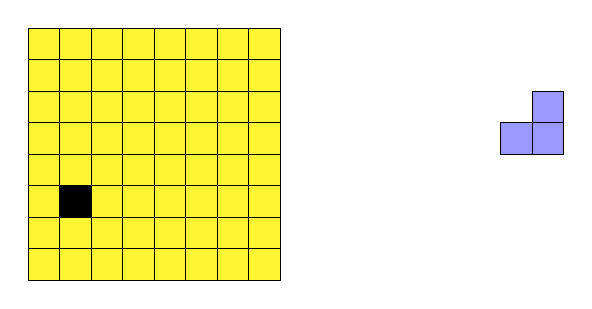
\begin{tikzpicture}[scale=0.4]
\filldraw[fill=yellow!80!white] (0,0) rectangle (8,8);
\draw[step=1cm,very thin] (0,0) grid (8,8);
\filldraw[fill=black] (1,2) rectangle (2,3);
%
\filldraw[fill=blue!40!white] (15,4)  rectangle (16,5);
\filldraw[fill=blue!40!white] (16,4)  rectangle (17,5);
\filldraw[fill=blue!40!white] (16,5)  rectangle (17,6);
%
\end{tikzpicture}
}
      
For full credit, your algorithms should take $O(n)$ time where $n=2^{2k}=(2^k)^2$ is the number of cells in the room.  The intent of the problem is to show that rooms of this kind can be tiled, do not worry about the
book-keeping needed to record the particular solution found by your divide and conquer algorithm.
\\
\\
\\
Continued on next page.
\newpage
\begin{algorithm}
    \item
    \begin{algorithmic}[1]
        \Procedure{Tiling}{$n$, $p$} \Comment{$n$ number of tiles, $p$ is missing cell}
        \If{$n$ = 2} \Comment{Base Case}
            \State Place tile around air vent
        \EndIf
        \State Place Tile in the center, but in such a way that it is not inside the $\frac{n}{2} \times \frac{n}{2}$ square that contains air vent 
        \State \Call{Tiling}{$\frac{n}{2}, p_1$}
        \State \Call{Tiling}{$\frac{n}{2}, p_2$}
        \State \Call{Tiling}{$\frac{n}{2}, p_3$}
        \State \Call{Tiling}{$\frac{n}{2}, p_4$}
        \EndProcedure
    \end{algorithmic}
    The base case will simply place an L-shaped tile wherever it goes and does not obstruct the air vent. If the square is greater than 2, then 
    the algorithm will place an L-shaped tile in the middle that covers $\frac{n}{2} \times \frac{n}{2}$ square that do not have the air vent. It will then recursively proceed to call on all $\frac{n}{2}$ 
    sized squares with each $p$ representing the empty square to be left out. 
\end{algorithm}   
\newpage
\begin{proofoc}
    \item
    \textbf{\textit{Base Case: }}$n=2$ \\
    When we have a $2 \times 2$ square, we can simply place the L-shaped tile around the air vent covering the entire $2 \times 2$ square.\\[0.7em]
    \textbf{\textit{Inductive Hypothesis: }}We will assume that this algorithm works for $2^k \times 2^k$ squares given that $k \geq 1$. \\[0.7em]
    \textbf{\textit{Inductive Step: }}I will try to prove that this algorithm works for a square of size $2^{k+1} \times 2^{k+1}$. When our algorithm begins, we place an L-shaped tile 
    in the middle of the $2^{k+1} \times 2^{k+1}$ square. When we begin our recursive calls, our first call we attempt to tile a $\frac{2^{k+1}}{2} \times \frac{2^{k+1}}{2}$ square.
    Mathematically, we know that:
    \begin{align*}
        \frac{2^{k+1}}{2} \times \frac{2^{k+1}}{2} & = \frac{2^k\times 2}{2} \times \frac{2^k\times 2}{2} \\
        & = 2^k \times 2^k
    \end{align*}
    Through our \textit{Inductive Hypothesis}, we can tile a $2^k \times 2^k$ square. Therfore, our induction is complete and we can conclude that our algorithm is correct. \\[1em]
    \textbf{\textit{Runtime Analysis: }}The algorithm recursively calls itself 4 times on $\frac{n}{2}$ sized squares each time, where $n$ is the dimension of the entire square, $2^k$. Our recurrence relation is then: 
    \begin{align*}
        T(n) = 4T(\frac{n}{2}) + \mathcal{O}(1)
    \end{align*}
    We add a constant because of the initial two comparisons that is done at the beginning of the algorithm that takes constant time. I will use Master's Theorem once again to show the runtime of 
    this algorithm. I will use coefficients $a=4$, $b=2$. I will also use case \#1:  
    \begin{align*}
        f(n) &= \mathcal{O}(n^{\log_ba}) \\
        T(n) & \leq \mathcal{O}(n^{\log_ba}) \\
        & \leq \mathcal{O}(n^{\log_24}) \\
        & \leq \mathcal{O}(n^2)
    \end{align*}
    We can conclude from Master's Theorem that this algorithm runs in $\mathcal{O}(n^2)$; however, I said that $n$ was equivalent to $2^k$, which is the dimension of the square. 
    This means that if we plug in my value for n, we get that the runtime is $\mathcal{O}((2^k)^2)$ or $\mathcal{O}(2^{2k})$. I can set $n = 2^2k$ since the total number of 
    tiles that we look at is $2^k \times 2^k = (2^k)^2$. Therefore, our algorithm runs in $\mathcal{O}(n)$. 
\end{proofoc}
\newpage
\end{enumerate}
\end{document}
